\documentclass[10pt,a4paper]{article}
\author{Elijah Andrews}
\usepackage[latin1]{inputenc}
\usepackage{amsmath}
\usepackage{amsfonts}
\usepackage{amssymb}
\usepackage[labelfont=bf]{caption}
\usepackage{graphicx}
\usepackage{csvsimple}
\usepackage[left=2cm,right=2cm,top=2cm,bottom=2cm]{geometry}
\usepackage{fancyhdr}
\usepackage[section]{placeins}
 
\pagestyle{fancy}
\fancyhf{}
\fancyhead[LE,RO]{Elijah Andrews}
\fancyhead[RE,LO]{Wing Aerodynamics Coursework}
\fancyfoot[CE,CO]{\leftmark}
\fancyfoot[LE,RO]{\thepage}

\makeatletter
\AtBeginDocument{%
  \expandafter\renewcommand\expandafter\subsection\expandafter{%
    \expandafter\@fb@secFB\subsection
  }%
}
\makeatother

\makeatletter
\AtBeginDocument{%
  \expandafter\renewcommand\expandafter\subsubsection\expandafter{%
    \expandafter\@fb@secFB\subsubsection
  }%
}
\makeatother

\makeatletter
\csvset{
  autotabularcenter/.style={
    file=#1,
    after head=\csv@pretable\begin{tabular}{|*{\csv@columncount}{c|}}\csv@tablehead,
    table head=\hline\csvlinetotablerow\\\hline,
    late after line=\\,
    table foot=\\\hline,
    late after last line=\csv@tablefoot\end{tabular}\csv@posttable,
    command=\csvlinetotablerow},
  autobooktabularcenter/.style={
    file=#1,
    after head=\csv@pretable\begin{tabular}{*{\csv@columncount}{c}}\csv@tablehead,
    table head=\toprule\csvlinetotablerow\\\midrule,
    late after line=\\,
    table foot=\\\bottomrule,
    late after last line=\csv@tablefoot\end{tabular}\csv@posttable,
    command=\csvlinetotablerow},
}
\makeatother
\newcommand{\csvautotabularcenter}[2][]{\csvloop{autotabularcenter={#2},#1}}
\newcommand{\csvautobooktabularcenter}[2][]{\csvloop{autobooktabularcenter={#2},#1}}

\usepackage{siunitx,array,booktabs}
\begin{document}
\textit{The code used in this coursework can be found at https://github.com/Xorgon/Wing-Aerodynamics-Coursework}
\section{Part I}
\subsection{Aerofoil Generation}
The Karman-Trefftz aerofoil properties assigned for this coursework were $\epsilon = 0.07$, $\beta = 0.02$, and $\tau = 0.15$. The aerofoil was generated using the provided MATLAB code and exported to a file. This file was then loaded in Python and the properties were measured using a computational algorithm (the algorithm can be found in `Python/graph\_aerofoils.py:95' in the `plot\_aerofoil' function). A camber line is first determined by taking the mean of the top and bottom surfaces. The function then sweeps along the calculated camber line and finds the maximum thickness and maximum thickness location. The properties calculated from this algorithm are found in the table in Figure \ref{fig:aerofoil property comparison}. The closest four digit NACA aerofoil is NACA 1511, also shown in Figure \ref{fig:aerofoil property comparison}. To verify that the algorithm for determining aerofoil properties is accurate, the same function has been run on the generated NACA 1511 aerofoil. The output from this calculation is shown as ``Measured NACA 1511" in Figure \ref{fig:aerofoil property comparison}. All of the properties are well within limits, if not exactly correct. This indicates that the measurements of the Karman-Trefftz aerofoil are highly likely to be accurate.
\\\\The aerofoils have also been plotted graphically in Figure \ref{fig:ktreff_naca_comparison}. Note that the y axis is not scaled exactly to the x axis, this is to allow for easier analysis of the differences as they are sufficiently similar that correctly scaled plots are almost indistinguishable. The aerofoil contour, camber line, and maximum thickness line are shown for both aerofoils. The camber line is virtually identical, however the Karman-Trefftz aerofoil is slightly thicker and has a maximum thickness position behind that of the NACA 1511. This has the effect of increasing the slope on the trailing half of the aerofoil contour. The effects of this difference are evident in later sections of this coursework.
\begin{figure}[!htb]
\begin{center}
\begin{tabular}{|c c c c|}
\hline
Property & Karman-Trefftz & NACA 1511 & Measured NACA 1511\\
\hline
Maximum Camber & 0.98\% & 1\% & 1\% \\
Maximum Camber Position & 49.50\% & 50\% & 50.1\% \\
Maximum Thickness & 11.43\% & 11\% & 11\%\\
Maximum Thickness Position & 33.03 \% & - & 30.83 \% \\
\hline
\end{tabular}
\end{center}
\caption{Aerofoil property comparison.}
\label{fig:aerofoil property comparison}
\end{figure}
\begin{figure}[!htb]
\centering
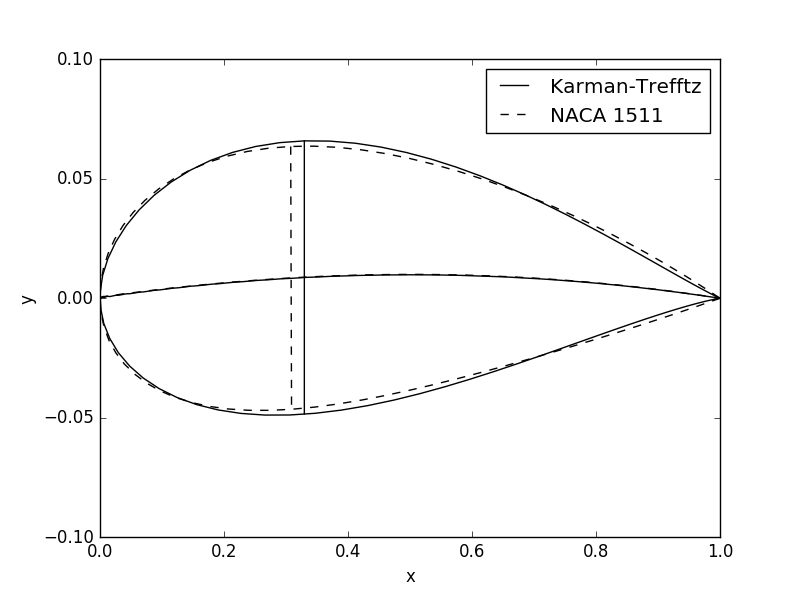
\includegraphics[scale=0.6]{Figures/ktreff_naca_comparison.png}
\caption{A comparison between a Karman-Trefftz aerofoil and its closest NACA aerofoil.}
\label{fig:ktreff_naca_comparison}
\end{figure}
\subsection{Parameter Variation}
\subsubsection{$\beta$ Variation}
The camber factor, $\beta$, is designed to vary the aerofoil camber. It is an angle that describes how the original circle is moved vertically in the complex plane. As $\beta$ increases, the original circle is moved upwards, thus increasing the camber of the transformed aerofoil.
\\As shown in Figure \ref{fig:beta_variation}, the maximum camber of an aerofoil increases a significant amount linearly with an increase in $\beta$. In addition, the maximum thickness increases with an increase in $\beta$, this relationship is not linear and is caused by the top surface getting higher faster than the lower surface. This increases the thickness as the camber increases. The change in thickness an be ignored, however, as it is negligibly small.
\begin{figure}[!htb]
\centering
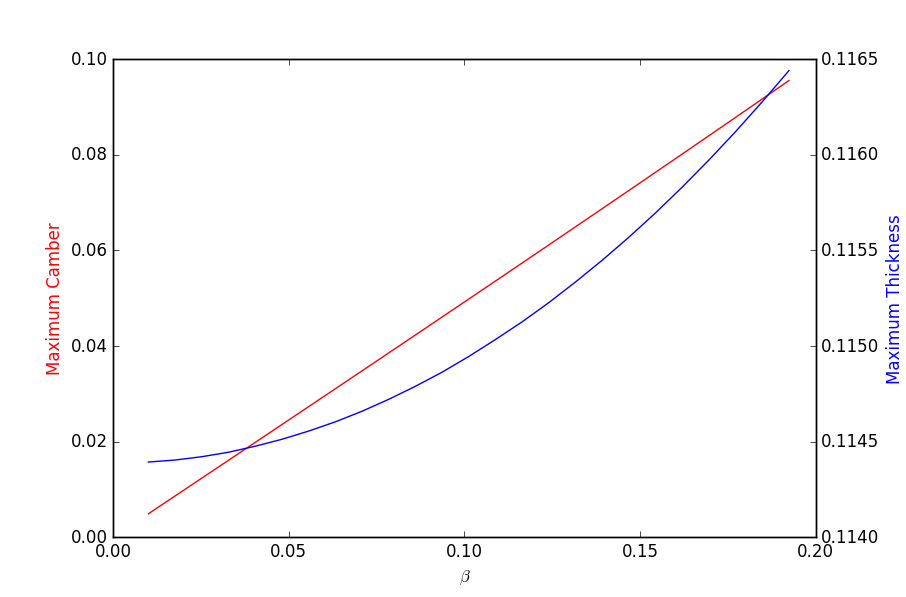
\includegraphics[scale=0.4925]{Figures/beta_variation.png}
\caption{How maximum thickness and maximum camber change with $\beta$.}
\label{fig:beta_variation}
\end{figure}
\subsubsection{$\epsilon$ Variation}
The thickness factor, $\epsilon$, is designed to vary the aerofoil thickness. It varies the horizontal offset of the original circle in the complex plane. As $\epsilon$ increases, the original circle is moved left, the further left the circle is, the thicker the transformed aerofoil.
\\As shown in Figure \ref{fig:epsilon_variation}, the maximum thickness increases a significant amount linearly with an increase in $\epsilon$. The camber also increases approximately linearly with an increase in $\epsilon$ but is a negligibly small change and so can be safely ignored.
\begin{figure}[!htb]
\centering
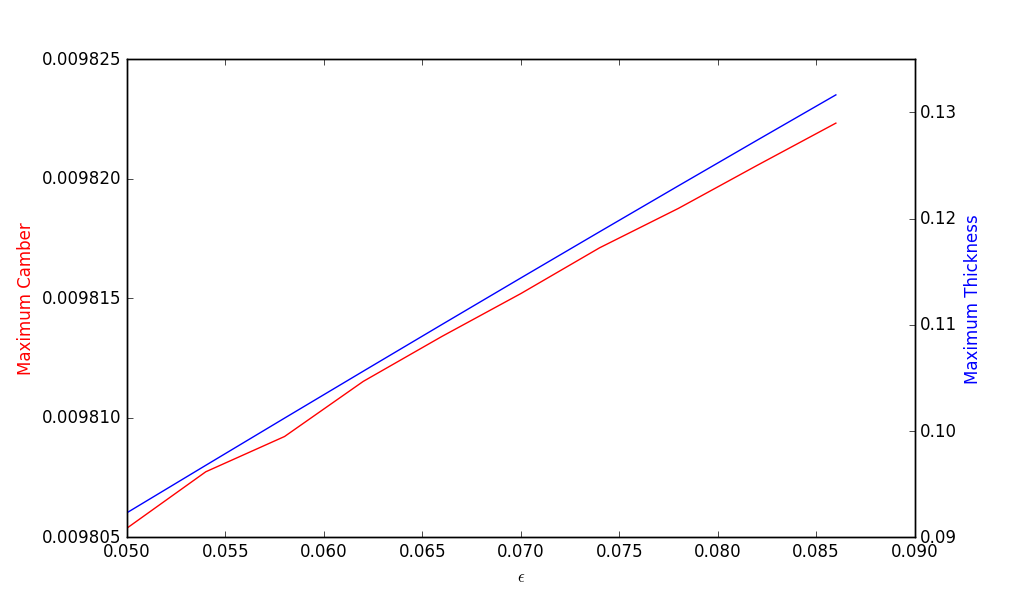
\includegraphics[scale=0.4925]{Figures/epsilon_variation.png}
\caption{How maximum thickness and maximum camber change with $\epsilon$.}
\label{fig:epsilon_variation}
\end{figure}
\section{Part II}
\subsection{Doublet Panel Method Accuracy}
The error formula is shown in Equation \ref{eq:error} where $h$ is the step, $n$ is the order of accuracy, and $C$ is some constant of proportionality. As shown, this can be rearranged to get the order of accuracy as the gradient of the graph of $log(Error)$ against $log(h)$ (Equation \ref{eq:accuracy order}). For the doublet panel method, the step is proportional to $1/N$ where $N$ is the number of panels used. Thus, the gradient of the graph of $log(Error)$ against $log(1/N)$ can be used to calculate the order of accuracy of the method.
\begin{align}
Error &= Ch^n \label{eq:error}
\\log(Error) &= log(Ch^n) \nonumber
\\log(Error) &= log(C) + nlog(h) \nonumber
\\n &= \dfrac{d(log(Error))}{d(log(h))} \label{eq:accuracy order}
\end{align}
Figure \ref{fig:accuracy} shows the plot of $log(Error)$ against $log(1/N)$, where $Error$ is the error in $C_L$ of the doublet panel code compared to the theoretical Karman-Trefftz aerofoil solution. The data shows that the doublet panel method doesn't have a uniform order of accuracy, however an approximate order of accuracy can be obtained from the best fit line. The best fit line has a gradient of 3.2, so the doublet panel method is approximately third order accurate.
\begin{figure}[!htb]
\centering
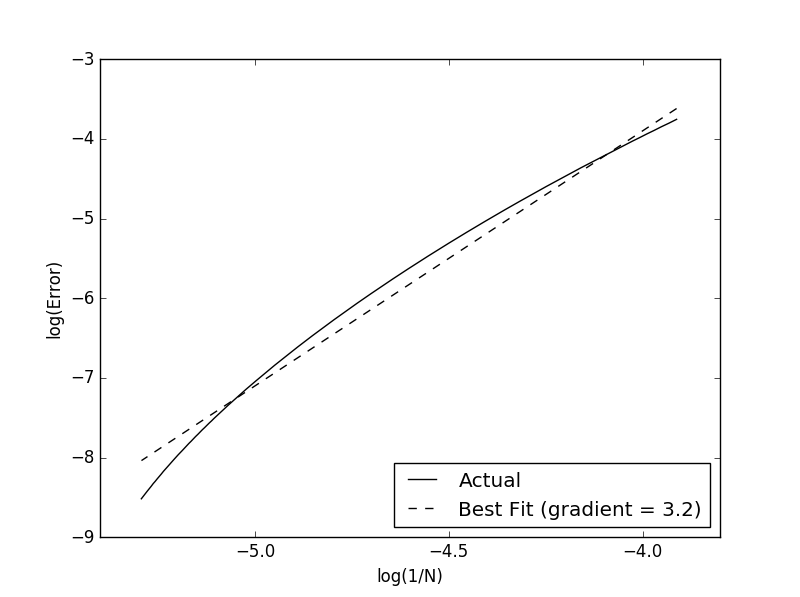
\includegraphics[scale=0.6]{Figures/accuracy.png}
\caption{Accuracy of the Doublet Panel Method.}
\label{fig:accuracy}
\end{figure}
\subsection{NACA and Karman-Trefftz Performance Comparison}
\subsubsection{Lift, Drag, and Stall Characteristics}
Figure \ref{fig:characteristics} shows the polar curve of the Karman-Trefftz and NACA 1511 aerofoils at varying angles of attack at $Re = 50e6$. The coefficient of lift ($C_L$) and coefficient of drag ($C_D$) characteristics follow the same trends as any other aerofoil. The NACA 1511 aerofoil has converged at angles beyond the stall, but these will be ignored as they are likely unphysical. When compared to the NACA 1511 aerofoil, the Karman-Trefftz aerofoil has a lower $C_L$ slope and a less steep drop-off in $C_L$ around the stall. In addition, the NACA 1511 aerofoil stalls marginally later than the Karman-Trefftz aerofoil. This is likely due to the Karman-Trefftz aerofoil having a steeper slope on the trailing half of the upper surface. The steeper slope requires the flow to turn a slightly sharper angle and so separates sooner. These effects are investigated further in the next sections.
\begin{figure}[!htb]
\centering
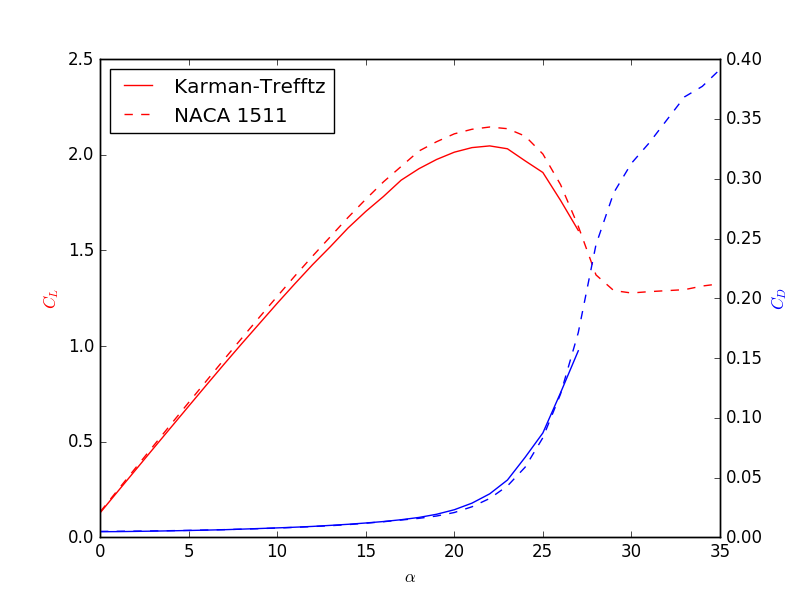
\includegraphics[scale=0.6]{Figures/polar_characteristics.png}
\caption{Lift, drag, and stall characteristics for the Karman-Trefftz and NACA 1511 aerofoils.}
\label{fig:characteristics}
\end{figure}
\subsubsection{Transition Position}
At some point along the surface of an aerofoil the flow transitions from laminar to turbulent. This increases drag but allows for higher flow turning angles and so later stalls. Figure \ref{fig:transition_comparison} shows how the transition point on the upper surface changes as the angle of attack changes at $Re = 50e6$. The NACA 1511 aerofoil transitions further forward than the Karman-Trefftz aerofoil at low angles of attack. This is likely due to the slightly higher initial curvature on the NACA 1511 compared with the Karman-Trefftz aerofoil (visible in Figure \ref{fig:ktreff_naca_comparison}). Beyond $\alpha = 3$ the Karman-Trefftz aerofoil has a transition point further forward, possibly due to the steeper gradient around the leading edge.
\begin{figure}[!htb]
\centering
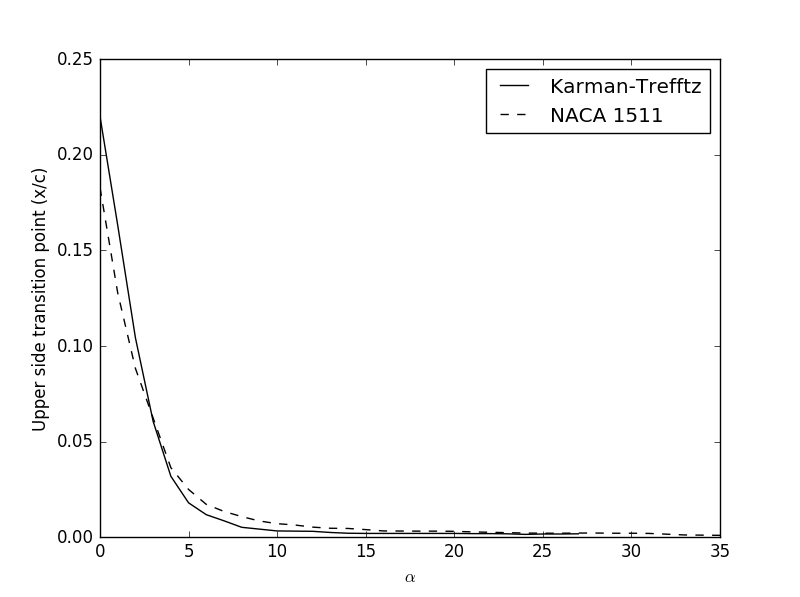
\includegraphics[scale=0.6]{Figures/transition_comparison.png}
\caption{Comparison of transition point between NACA 1511 and Karman-Trefftz aerofoils.}
\label{fig:transition_comparison}
\end{figure}
\subsubsection{Separation Position}
To efficiently analyse the separation point of each aerofoil, code was written to detect the separation point based on the upper surface pressure distribution (this code can be found in `Python/run\_xfoil.py:74' in the `calculate\_separation\_point' function). As shown in Figure \ref{fig:separation_point}, the separation point corresponds to a pressure inversion on the upper surface of the aerofoil. This inversion can be detected by measuring the pressure gradient along the aerofoil.
\\\\Figure \ref{fig:separation_comparison} shows how the separation point changes with angle of attack. In general, the separation point moves forward along the aerofoil as the angle of attack increases. As expected, separation is not present at low angles of attack. The onset of separation is earlier on the Karman-Trefftz aerofoil, this is likely due to the steeper trailing half gradient on the upper surface that has been mentioned before. Both the Karman-Trefftz and the NACA 1511 share a similar decrease in separation point as the angle of attack increases up to the point at which the flow simulation no longer converges.
\begin{figure}[!htb]
\centering
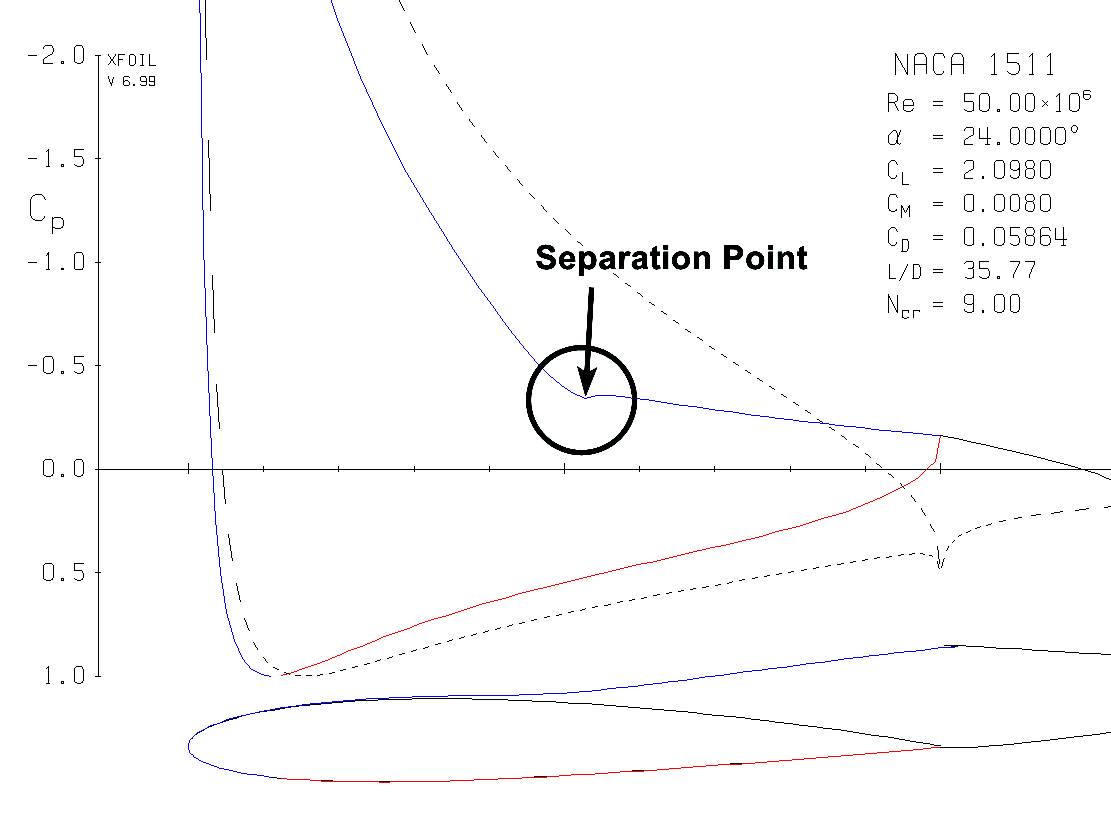
\includegraphics[scale=0.35]{Figures/separation_point.png}
\caption{The definition of the separation point used in this coursework.}
\label{fig:separation_point}
\end{figure}
\begin{figure}[!htb]
\centering
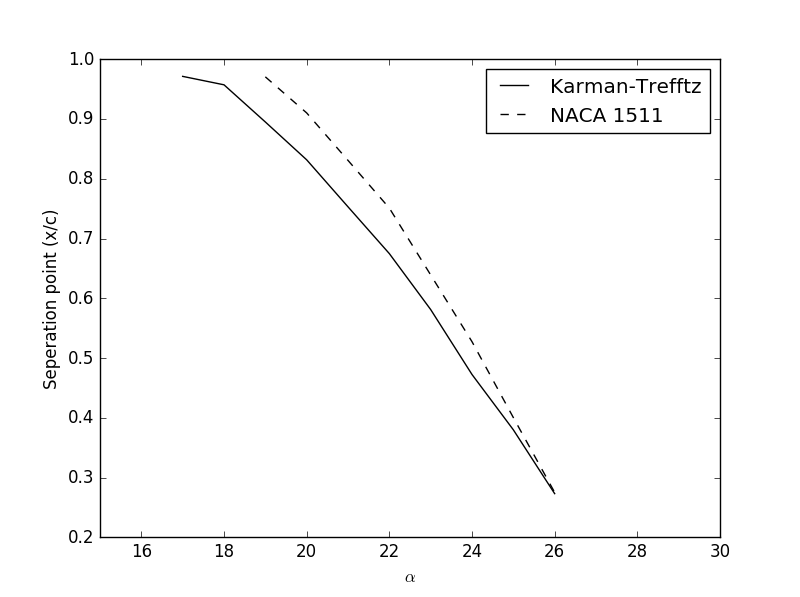
\includegraphics[scale=0.55]{Figures/separation_comparison.png}
\caption{Comparison of separation point between NACA 1511 and Karman-Trefftz aerofoils.}
\label{fig:separation_comparison}
\end{figure}
\end{document}
